\documentclass[1p]{elsarticle_modified}
%\bibliographystyle{elsarticle-num}

%\usepackage[colorlinks]{hyperref}
%\usepackage{abbrmath_seonhwa} %\Abb, \Ascr, \Acal ,\Abf, \Afrak
\usepackage{amsfonts}
\usepackage{amssymb}
\usepackage{amsmath}
\usepackage{amsthm}
\usepackage{scalefnt}
\usepackage{amsbsy}
\usepackage{kotex}
\usepackage{caption}
\usepackage{subfig}
\usepackage{color}
\usepackage{graphicx}
\usepackage{xcolor} %% white, black, red, green, blue, cyan, magenta, yellow
\usepackage{float}
\usepackage{setspace}
\usepackage{hyperref}

\usepackage{tikz}
\usetikzlibrary{arrows}

\usepackage{multirow}
\usepackage{array} % fixed length table
\usepackage{hhline}

%%%%%%%%%%%%%%%%%%%%%
\makeatletter
\renewcommand*\env@matrix[1][\arraystretch]{%
	\edef\arraystretch{#1}%
	\hskip -\arraycolsep
	\let\@ifnextchar\new@ifnextchar
	\array{*\c@MaxMatrixCols c}}
\makeatother %https://tex.stackexchange.com/questions/14071/how-can-i-increase-the-line-spacing-in-a-matrix
%%%%%%%%%%%%%%%

\usepackage[normalem]{ulem}

\newcommand{\msout}[1]{\ifmmode\text{\sout{\ensuremath{#1}}}\else\sout{#1}\fi}
%SOURCE: \msout is \stkout macro in https://tex.stackexchange.com/questions/20609/strikeout-in-math-mode

\newcommand{\cancel}[1]{
	\ifmmode
	{\color{red}\msout{#1}}
	\else
	{\color{red}\sout{#1}}
	\fi
}

\newcommand{\add}[1]{
	{\color{blue}\uwave{#1}}
}

\newcommand{\replace}[2]{
	\ifmmode
	{\color{red}\msout{#1}}{\color{blue}\uwave{#2}}
	\else
	{\color{red}\sout{#1}}{\color{blue}\uwave{#2}}
	\fi
}

\newcommand{\Sol}{\mathcal{S}} %segment
\newcommand{\D}{D} %diagram
\newcommand{\A}{\mathcal{A}} %arc


%%%%%%%%%%%%%%%%%%%%%%%%%%%%%5 test

\def\sl{\operatorname{\textup{SL}}(2,\Cbb)}
\def\psl{\operatorname{\textup{PSL}}(2,\Cbb)}
\def\quan{\mkern 1mu \triangleright \mkern 1mu}

\theoremstyle{definition}
\newtheorem{thm}{Theorem}[section]
\newtheorem{prop}[thm]{Proposition}
\newtheorem{lem}[thm]{Lemma}
\newtheorem{ques}[thm]{Question}
\newtheorem{cor}[thm]{Corollary}
\newtheorem{defn}[thm]{Definition}
\newtheorem{exam}[thm]{Example}
\newtheorem{rmk}[thm]{Remark}
\newtheorem{alg}[thm]{Algorithm}

\newcommand{\I}{\sqrt{-1}}
\begin{document}

%\begin{frontmatter}
%
%\title{Boundary parabolic representations of knots up to 8 crossings}
%
%%% Group authors per affiliation:
%\author{Yunhi Cho} 
%\address{Department of Mathematics, University of Seoul, Seoul, Korea}
%\ead{yhcho@uos.ac.kr}
%
%
%\author{Seonhwa Kim} %\fnref{s_kim}}
%\address{Center for Geometry and Physics, Institute for Basic Science, Pohang, 37673, Korea}
%\ead{ryeona17@ibs.re.kr}
%
%\author{Hyuk Kim}
%\address{Department of Mathematical Sciences, Seoul National University, Seoul 08826, Korea}
%\ead{hyukkim@snu.ac.kr}
%
%\author{Seokbeom Yoon}
%\address{Department of Mathematical Sciences, Seoul National University, Seoul, 08826,  Korea}
%\ead{sbyoon15@snu.ac.kr}
%
%\begin{abstract}
%We find all boundary parabolic representation of knots up to 8 crossings.
%
%\end{abstract}
%\begin{keyword}
%    \MSC[2010] 57M25 
%\end{keyword}
%
%\end{frontmatter}

%\linenumbers
%\tableofcontents
%
\newcommand\colored[1]{\textcolor{white}{\rule[-0.35ex]{0.8em}{1.4ex}}\kern-0.8em\color{red} #1}%
%\newcommand\colored[1]{\textcolor{white}{ #1}\kern-2.17ex	\textcolor{white}{ #1}\kern-1.81ex	\textcolor{white}{ #1}\kern-2.15ex\color{red}#1	}

{\Large $\underline{11a_{61}~(K11a_{61})}$}

\setlength{\tabcolsep}{10pt}
\renewcommand{\arraystretch}{1.6}
\vspace{1cm}\begin{tabular}{m{100pt}>{\centering\arraybackslash}m{274pt}}
\multirow{5}{120pt}{
	\centering
	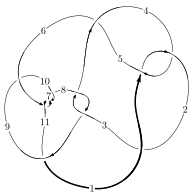
\includegraphics[width=112pt]{../../../GIT/diagram.site/Diagrams/png/310_11a_61.png}\\
\ \ \ A knot diagram\footnotemark}&
\allowdisplaybreaks
\textbf{Linearized knot diagam} \\
\cline{2-2}
 &
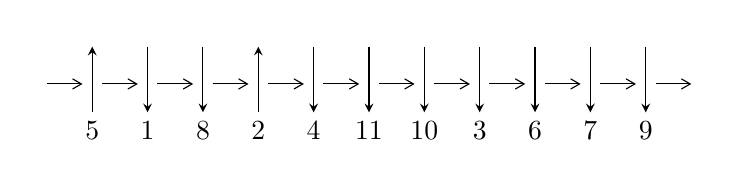
\begin{tikzpicture}[x=20pt, y=17pt]
	% nodes
	\node (C0) at (0, 0) {};
	\node (C1) at (1, 0) {};
	\node (C1U) at (1, +1) {};
	\node (C1D) at (1, -1) {5};

	\node (C2) at (2, 0) {};
	\node (C2U) at (2, +1) {};
	\node (C2D) at (2, -1) {1};

	\node (C3) at (3, 0) {};
	\node (C3U) at (3, +1) {};
	\node (C3D) at (3, -1) {8};

	\node (C4) at (4, 0) {};
	\node (C4U) at (4, +1) {};
	\node (C4D) at (4, -1) {2};

	\node (C5) at (5, 0) {};
	\node (C5U) at (5, +1) {};
	\node (C5D) at (5, -1) {4};

	\node (C6) at (6, 0) {};
	\node (C6U) at (6, +1) {};
	\node (C6D) at (6, -1) {11};

	\node (C7) at (7, 0) {};
	\node (C7U) at (7, +1) {};
	\node (C7D) at (7, -1) {10};

	\node (C8) at (8, 0) {};
	\node (C8U) at (8, +1) {};
	\node (C8D) at (8, -1) {3};

	\node (C9) at (9, 0) {};
	\node (C9U) at (9, +1) {};
	\node (C9D) at (9, -1) {6};

	\node (C10) at (10, 0) {};
	\node (C10U) at (10, +1) {};
	\node (C10D) at (10, -1) {7};

	\node (C11) at (11, 0) {};
	\node (C11U) at (11, +1) {};
	\node (C11D) at (11, -1) {9};
	\node (C12) at (12, 0) {};

	% arrows
	\draw[->,>={angle 60}]
	(C0) edge (C1) (C1) edge (C2) (C2) edge (C3) (C3) edge (C4) (C4) edge (C5) (C5) edge (C6) (C6) edge (C7) (C7) edge (C8) (C8) edge (C9) (C9) edge (C10) (C10) edge (C11) (C11) edge (C12) ;	\draw[->,>=stealth]
	(C1D) edge (C1U) (C2U) edge (C2D) (C3U) edge (C3D) (C4D) edge (C4U) (C5U) edge (C5D) (C6U) edge (C6D) (C7U) edge (C7D) (C8U) edge (C8D) (C9U) edge (C9D) (C10U) edge (C10D) (C11U) edge (C11D) ;
	\end{tikzpicture} \\
\hhline{~~} \\& 
\textbf{Solving Sequence} \\ \cline{2-2} 
 &
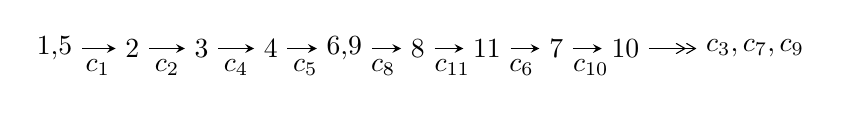
\begin{tikzpicture}[x=25pt, y=7pt]
	% node
	\node (A0) at (-1/8, 0) {1,5};
	\node (A1) at (1, 0) {2};
	\node (A2) at (2, 0) {3};
	\node (A3) at (3, 0) {4};
	\node (A4) at (65/16, 0) {6,9};
	\node (A5) at (41/8, 0) {8};
	\node (A6) at (49/8, 0) {11};
	\node (A7) at (57/8, 0) {7};
	\node (A8) at (65/8, 0) {10};
	\node (C1) at (1/2, -1) {$c_{1}$};
	\node (C2) at (3/2, -1) {$c_{2}$};
	\node (C3) at (5/2, -1) {$c_{4}$};
	\node (C4) at (7/2, -1) {$c_{5}$};
	\node (C5) at (37/8, -1) {$c_{8}$};
	\node (C6) at (45/8, -1) {$c_{11}$};
	\node (C7) at (53/8, -1) {$c_{6}$};
	\node (C8) at (61/8, -1) {$c_{10}$};
	\node (A9) at (10, 0) {$c_{3},c_{7},c_{9}$};

	% edge
	\draw[->,>=stealth]	
	(A0) edge (A1) (A1) edge (A2) (A2) edge (A3) (A3) edge (A4) (A4) edge (A5) (A5) edge (A6) (A6) edge (A7) (A7) edge (A8) ;
	\draw[->>,>={angle 60}]	
	(A8) edge (A9);
\end{tikzpicture} \\ 

\end{tabular} \\

\footnotetext{
The image of knot diagram is generated by the software ``\textbf{Draw programme}" developed by Andrew Bartholomew(\url{http://www.layer8.co.uk/maths/draw/index.htm\#Running-draw}), where we modified some parts for our purpose(\url{https://github.com/CATsTAILs/LinksPainter}).
}\phantom \\ \newline 
\centering \textbf{Ideals for irreducible components\footnotemark of $X_{\text{par}}$} 
 
\begin{align*}
I^u_{1}&=\langle 
8 u^{56}-9 u^{55}+\cdots+4 b-7,\;11 u^{56}-40 u^{55}+\cdots+4 a+1,\;u^{57}-4 u^{56}+\cdots+7 u-1\rangle \\
I^u_{2}&=\langle 
- a u+b,\;a^3+a^2 u+a^2+1,\;u^2+u+1\rangle \\
\\
\end{align*}
\raggedright * 2 irreducible components of $\dim_{\mathbb{C}}=0$, with total 63 representations.\\
\footnotetext{All coefficients of polynomials are rational numbers. But the coefficients are sometimes approximated in decimal forms when there is not enough margin.}
\newpage
\renewcommand{\arraystretch}{1}
\centering \section*{I. $I^u_{1}= \langle 8 u^{56}-9 u^{55}+\cdots+4 b-7,\;11 u^{56}-40 u^{55}+\cdots+4 a+1,\;u^{57}-4 u^{56}+\cdots+7 u-1 \rangle$}
\flushleft \textbf{(i) Arc colorings}\\
\begin{tabular}{m{7pt} m{180pt} m{7pt} m{180pt} }
\flushright $a_{1}=$&$\begin{pmatrix}1\\0\end{pmatrix}$ \\
\flushright $a_{5}=$&$\begin{pmatrix}0\\u\end{pmatrix}$ \\
\flushright $a_{2}=$&$\begin{pmatrix}1\\- u^2\end{pmatrix}$ \\
\flushright $a_{3}=$&$\begin{pmatrix}u^2+1\\- u^2\end{pmatrix}$ \\
\flushright $a_{4}=$&$\begin{pmatrix}- u\\u^3+u\end{pmatrix}$ \\
\flushright $a_{6}=$&$\begin{pmatrix}- u^3\\u^5+u^3+u\end{pmatrix}$ \\
\flushright $a_{9}=$&$\begin{pmatrix}-\frac{11}{4} u^{56}+10 u^{55}+\cdots+\frac{67}{4} u-\frac{1}{4}\\-2 u^{56}+\frac{9}{4} u^{55}+\cdots-11 u+\frac{7}{4}\end{pmatrix}$ \\
\flushright $a_{8}=$&$\begin{pmatrix}-\frac{9}{4} u^{56}+16 u^{55}+\cdots+\frac{189}{4} u-\frac{23}{4}\\-7 u^{56}+\frac{55}{4} u^{55}+\cdots-10 u+\frac{9}{4}\end{pmatrix}$ \\
\flushright $a_{11}=$&$\begin{pmatrix}-\frac{1}{4} u^{56}+\frac{3}{4} u^{55}+\cdots+\frac{13}{4} u+2\\\frac{1}{4} u^{56}- u^{55}+\cdots-\frac{11}{4} u+\frac{1}{4}\end{pmatrix}$ \\
\flushright $a_{7}=$&$\begin{pmatrix}\frac{11}{4} u^{56}-\frac{47}{4} u^{55}+\cdots-\frac{121}{4} u+4\\\frac{3}{4} u^{56}+\frac{1}{4} u^{55}+\cdots+\frac{59}{4} u-\frac{5}{2}\end{pmatrix}$ \\
\flushright $a_{10}=$&$\begin{pmatrix}-\frac{7}{4} u^{56}+\frac{63}{4} u^{55}+\cdots+\frac{223}{4} u-7\\-7 u^{56}+\frac{57}{4} u^{55}+\cdots-12 u+\frac{11}{4}\end{pmatrix}$\\ \flushright $a_{10}=$&$\begin{pmatrix}-\frac{7}{4} u^{56}+\frac{63}{4} u^{55}+\cdots+\frac{223}{4} u-7\\-7 u^{56}+\frac{57}{4} u^{55}+\cdots-12 u+\frac{11}{4}\end{pmatrix}$\\&\end{tabular}
\flushleft \textbf{(ii) Obstruction class $= -1$}\\~\\
\flushleft \textbf{(iii) Cusp Shapes $= -8 u^{56}+\frac{25}{2} u^{55}+\cdots-20 u-7$}\\~\\
\newpage\renewcommand{\arraystretch}{1}
\flushleft \textbf{(iv) u-Polynomials at the component}\newline \\
\begin{tabular}{m{50pt}|m{274pt}}
Crossings & \hspace{64pt}u-Polynomials at each crossing \\
\hline $$\begin{aligned}c_{1},c_{4}\end{aligned}$$&$\begin{aligned}
&u^{57}+4 u^{56}+\cdots+7 u+1
\end{aligned}$\\
\hline $$\begin{aligned}c_{2},c_{5}\end{aligned}$$&$\begin{aligned}
&u^{57}+18 u^{56}+\cdots+23 u-1
\end{aligned}$\\
\hline $$\begin{aligned}c_{3},c_{8}\end{aligned}$$&$\begin{aligned}
&u^{57}+u^{56}+\cdots+160 u+64
\end{aligned}$\\
\hline $$\begin{aligned}c_{6},c_{7},c_{10}\end{aligned}$$&$\begin{aligned}
&u^{57}-3 u^{56}+\cdots-6 u+1
\end{aligned}$\\
\hline $$\begin{aligned}c_{9}\end{aligned}$$&$\begin{aligned}
&u^{57}+3 u^{56}+\cdots-624 u+73
\end{aligned}$\\
\hline $$\begin{aligned}c_{11}\end{aligned}$$&$\begin{aligned}
&u^{57}-11 u^{56}+\cdots-2040 u+209
\end{aligned}$\\
\hline
\end{tabular}\\~\\
\newpage\renewcommand{\arraystretch}{1}
\flushleft \textbf{(v) Riley Polynomials at the component}\newline \\
\begin{tabular}{m{50pt}|m{274pt}}
Crossings & \hspace{64pt}Riley Polynomials at each crossing \\
\hline $$\begin{aligned}c_{1},c_{4}\end{aligned}$$&$\begin{aligned}
&y^{57}+18 y^{56}+\cdots+23 y-1
\end{aligned}$\\
\hline $$\begin{aligned}c_{2},c_{5}\end{aligned}$$&$\begin{aligned}
&y^{57}+46 y^{56}+\cdots+1015 y-1
\end{aligned}$\\
\hline $$\begin{aligned}c_{3},c_{8}\end{aligned}$$&$\begin{aligned}
&y^{57}+35 y^{56}+\cdots-39936 y-4096
\end{aligned}$\\
\hline $$\begin{aligned}c_{6},c_{7},c_{10}\end{aligned}$$&$\begin{aligned}
&y^{57}+53 y^{56}+\cdots+6 y-1
\end{aligned}$\\
\hline $$\begin{aligned}c_{9}\end{aligned}$$&$\begin{aligned}
&y^{57}+9 y^{56}+\cdots-41762 y-5329
\end{aligned}$\\
\hline $$\begin{aligned}c_{11}\end{aligned}$$&$\begin{aligned}
&y^{57}+29 y^{56}+\cdots-624082 y-43681
\end{aligned}$\\
\hline
\end{tabular}\\~\\
\newpage\flushleft \textbf{(vi) Complex Volumes and Cusp Shapes}
$$\begin{array}{c|c|c}  
\text{Solutions to }I^u_{1}& \I (\text{vol} + \sqrt{-1}CS) & \text{Cusp shape}\\
 \hline 
\begin{aligned}
u &= -0.411000 + 0.945370 I \\
a &= \phantom{-}0.758571 + 0.375458 I \\
b &= -0.159926 + 0.346294 I\end{aligned}
 & -0.43337 - 1.68301 I & -2.91269 + 0. I\phantom{ +0.000000I} \\ \hline\begin{aligned}
u &= -0.411000 - 0.945370 I \\
a &= \phantom{-}0.758571 - 0.375458 I \\
b &= -0.159926 - 0.346294 I\end{aligned}
 & -0.43337 + 1.68301 I & -2.91269 + 0. I\phantom{ +0.000000I} \\ \hline\begin{aligned}
u &= -0.070350 + 0.957209 I \\
a &= \phantom{-}0.843157 + 0.528242 I \\
b &= \phantom{-}1.012250 + 0.111658 I\end{aligned}
 & -0.22072 - 2.23623 I & -9.39240 + 3.87464 I \\ \hline\begin{aligned}
u &= -0.070350 - 0.957209 I \\
a &= \phantom{-}0.843157 - 0.528242 I \\
b &= \phantom{-}1.012250 - 0.111658 I\end{aligned}
 & -0.22072 + 2.23623 I & -9.39240 - 3.87464 I \\ \hline\begin{aligned}
u &= -0.294254 + 0.900156 I \\
a &= \phantom{-}0.889838 + 0.254291 I \\
b &= \phantom{-}0.192184 + 0.303495 I\end{aligned}
 & -0.43103 - 1.63888 I & -4.79988 + 2.71199 I \\ \hline\begin{aligned}
u &= -0.294254 - 0.900156 I \\
a &= \phantom{-}0.889838 - 0.254291 I \\
b &= \phantom{-}0.192184 - 0.303495 I\end{aligned}
 & -0.43103 + 1.63888 I & -4.79988 - 2.71199 I \\ \hline\begin{aligned}
u &= \phantom{-}0.716145 + 0.819187 I \\
a &= -0.945498 + 0.434435 I \\
b &= \phantom{-}1.40998 + 0.63877 I\end{aligned}
 & \phantom{-}4.56397 - 1.17086 I & \phantom{-0.000000 } 0 \\ \hline\begin{aligned}
u &= \phantom{-}0.716145 - 0.819187 I \\
a &= -0.945498 - 0.434435 I \\
b &= \phantom{-}1.40998 - 0.63877 I\end{aligned}
 & \phantom{-}4.56397 + 1.17086 I & \phantom{-0.000000 } 0 \\ \hline\begin{aligned}
u &= -0.722279 + 0.830660 I \\
a &= \phantom{-}1.00866 - 1.56975 I \\
b &= -0.112045 + 0.922007 I\end{aligned}
 & \phantom{-}1.73223 - 1.00864 I & -7.00000 + 0. I\phantom{ +0.000000I} \\ \hline\begin{aligned}
u &= -0.722279 - 0.830660 I \\
a &= \phantom{-}1.00866 + 1.56975 I \\
b &= -0.112045 - 0.922007 I\end{aligned}
 & \phantom{-}1.73223 + 1.00864 I & -7.00000 + 0. I\phantom{ +0.000000I}\\
 \hline 
 \end{array}$$\newpage$$\begin{array}{c|c|c}  
\text{Solutions to }I^u_{1}& \I (\text{vol} + \sqrt{-1}CS) & \text{Cusp shape}\\
 \hline 
\begin{aligned}
u &= -0.221111 + 1.079490 I \\
a &= -0.821842 - 0.181447 I \\
b &= -0.613293 - 1.011210 I\end{aligned}
 & -1.42166 - 4.84212 I & -7.00000 + 7.62059 I \\ \hline\begin{aligned}
u &= -0.221111 - 1.079490 I \\
a &= -0.821842 + 0.181447 I \\
b &= -0.613293 + 1.011210 I\end{aligned}
 & -1.42166 + 4.84212 I & -7.00000 - 7.62059 I \\ \hline\begin{aligned}
u &= \phantom{-}0.864422 + 0.721606 I \\
a &= \phantom{-}0.74235 + 1.40599 I \\
b &= -0.62330 - 1.47673 I\end{aligned}
 & \phantom{-}5.87637 - 4.55093 I & \phantom{-0.000000 } 0 \\ \hline\begin{aligned}
u &= \phantom{-}0.864422 - 0.721606 I \\
a &= \phantom{-}0.74235 - 1.40599 I \\
b &= -0.62330 + 1.47673 I\end{aligned}
 & \phantom{-}5.87637 + 4.55093 I & \phantom{-0.000000 } 0 \\ \hline\begin{aligned}
u &= \phantom{-}0.710335 + 0.874003 I \\
a &= \phantom{-}0.541401 - 0.977846 I \\
b &= -1.50306 - 0.11683 I\end{aligned}
 & \phantom{-}0.69484 + 2.72065 I & \phantom{-0.000000 } 0 \\ \hline\begin{aligned}
u &= \phantom{-}0.710335 - 0.874003 I \\
a &= \phantom{-}0.541401 + 0.977846 I \\
b &= -1.50306 + 0.11683 I\end{aligned}
 & \phantom{-}0.69484 - 2.72065 I & \phantom{-0.000000 } 0 \\ \hline\begin{aligned}
u &= -0.782668 + 0.823558 I \\
a &= -1.38003 + 1.86072 I \\
b &= \phantom{-}0.318434 - 1.211320 I\end{aligned}
 & \phantom{-}7.55130 + 1.74072 I & \phantom{-0.000000 } 0 \\ \hline\begin{aligned}
u &= -0.782668 - 0.823558 I \\
a &= -1.38003 - 1.86072 I \\
b &= \phantom{-}0.318434 + 1.211320 I\end{aligned}
 & \phantom{-}7.55130 - 1.74072 I & \phantom{-0.000000 } 0 \\ \hline\begin{aligned}
u &= \phantom{-}0.846418 + 0.761999 I \\
a &= -0.471724 - 1.032250 I \\
b &= \phantom{-}0.571036 + 1.197990 I\end{aligned}
 & \phantom{-}6.72836 - 0.26468 I & \phantom{-0.000000 } 0 \\ \hline\begin{aligned}
u &= \phantom{-}0.846418 - 0.761999 I \\
a &= -0.471724 + 1.032250 I \\
b &= \phantom{-}0.571036 - 1.197990 I\end{aligned}
 & \phantom{-}6.72836 + 0.26468 I & \phantom{-0.000000 } 0\\
 \hline 
 \end{array}$$\newpage$$\begin{array}{c|c|c}  
\text{Solutions to }I^u_{1}& \I (\text{vol} + \sqrt{-1}CS) & \text{Cusp shape}\\
 \hline 
\begin{aligned}
u &= \phantom{-}0.892838 + 0.709779 I \\
a &= -0.72817 - 1.72293 I \\
b &= \phantom{-}0.54713 + 1.65321 I\end{aligned}
 & \phantom{-}11.7431 - 8.1696 I & \phantom{-0.000000 } 0 \\ \hline\begin{aligned}
u &= \phantom{-}0.892838 - 0.709779 I \\
a &= -0.72817 + 1.72293 I \\
b &= \phantom{-}0.54713 - 1.65321 I\end{aligned}
 & \phantom{-}11.7431 + 8.1696 I & \phantom{-0.000000 } 0 \\ \hline\begin{aligned}
u &= -0.579065 + 0.988208 I \\
a &= -0.527800 - 1.214050 I \\
b &= \phantom{-}0.733184 + 0.166462 I\end{aligned}
 & \phantom{-}2.70688 - 3.25300 I & \phantom{-0.000000 } 0 \\ \hline\begin{aligned}
u &= -0.579065 - 0.988208 I \\
a &= -0.527800 + 1.214050 I \\
b &= \phantom{-}0.733184 - 0.166462 I\end{aligned}
 & \phantom{-}2.70688 + 3.25300 I & \phantom{-0.000000 } 0 \\ \hline\begin{aligned}
u &= \phantom{-}0.046272 + 0.846532 I \\
a &= -1.18927 - 0.76890 I \\
b &= -0.905005 + 0.577259 I\end{aligned}
 & -2.85410 + 0.74308 I & -13.57323 - 1.00600 I \\ \hline\begin{aligned}
u &= \phantom{-}0.046272 - 0.846532 I \\
a &= -1.18927 + 0.76890 I \\
b &= -0.905005 - 0.577259 I\end{aligned}
 & -2.85410 - 0.74308 I & -13.57323 + 1.00600 I \\ \hline\begin{aligned}
u &= -0.234257 + 1.130480 I \\
a &= \phantom{-}0.840745 + 0.057014 I \\
b &= \phantom{-}0.59116 + 1.34495 I\end{aligned}
 & \phantom{-}4.07584 - 8.10637 I & \phantom{-0.000000 } 0 \\ \hline\begin{aligned}
u &= -0.234257 - 1.130480 I \\
a &= \phantom{-}0.840745 - 0.057014 I \\
b &= \phantom{-}0.59116 - 1.34495 I\end{aligned}
 & \phantom{-}4.07584 + 8.10637 I & \phantom{-0.000000 } 0 \\ \hline\begin{aligned}
u &= -0.386185 + 1.092590 I \\
a &= -1.129960 - 0.354062 I \\
b &= \phantom{-}0.360548 - 1.019790 I\end{aligned}
 & \phantom{-}5.00981 + 0.63384 I & \phantom{-0.000000 } 0 \\ \hline\begin{aligned}
u &= -0.386185 - 1.092590 I \\
a &= -1.129960 + 0.354062 I \\
b &= \phantom{-}0.360548 + 1.019790 I\end{aligned}
 & \phantom{-}5.00981 - 0.63384 I & \phantom{-0.000000 } 0\\
 \hline 
 \end{array}$$\newpage$$\begin{array}{c|c|c}  
\text{Solutions to }I^u_{1}& \I (\text{vol} + \sqrt{-1}CS) & \text{Cusp shape}\\
 \hline 
\begin{aligned}
u &= -0.718160 + 0.909667 I \\
a &= -0.49430 + 1.92093 I \\
b &= -0.337710 - 1.036600 I\end{aligned}
 & \phantom{-}1.48928 - 4.49756 I & \phantom{-0.000000 } 0 \\ \hline\begin{aligned}
u &= -0.718160 - 0.909667 I \\
a &= -0.49430 - 1.92093 I \\
b &= -0.337710 + 1.036600 I\end{aligned}
 & \phantom{-}1.48928 + 4.49756 I & \phantom{-0.000000 } 0 \\ \hline\begin{aligned}
u &= \phantom{-}0.711635 + 0.923729 I \\
a &= -0.071999 + 1.393300 I \\
b &= \phantom{-}1.46379 - 0.43402 I\end{aligned}
 & \phantom{-}4.23779 + 6.64103 I & \phantom{-0.000000 } 0 \\ \hline\begin{aligned}
u &= \phantom{-}0.711635 - 0.923729 I \\
a &= -0.071999 - 1.393300 I \\
b &= \phantom{-}1.46379 + 0.43402 I\end{aligned}
 & \phantom{-}4.23779 - 6.64103 I & \phantom{-0.000000 } 0 \\ \hline\begin{aligned}
u &= \phantom{-}0.145913 + 0.817129 I \\
a &= \phantom{-}1.44787 + 1.01076 I \\
b &= \phantom{-}0.884513 - 1.043560 I\end{aligned}
 & \phantom{-}1.92041 + 4.01720 I & -8.21820 - 1.67425 I \\ \hline\begin{aligned}
u &= \phantom{-}0.145913 - 0.817129 I \\
a &= \phantom{-}1.44787 - 1.01076 I \\
b &= \phantom{-}0.884513 + 1.043560 I\end{aligned}
 & \phantom{-}1.92041 - 4.01720 I & -8.21820 + 1.67425 I \\ \hline\begin{aligned}
u &= -0.610136 + 0.543922 I \\
a &= -1.393620 + 0.207735 I \\
b &= \phantom{-}0.544710 + 0.046272 I\end{aligned}
 & \phantom{-}3.98401 - 1.43384 I & -1.02074 + 3.18853 I \\ \hline\begin{aligned}
u &= -0.610136 - 0.543922 I \\
a &= -1.393620 - 0.207735 I \\
b &= \phantom{-}0.544710 - 0.046272 I\end{aligned}
 & \phantom{-}3.98401 + 1.43384 I & -1.02074 - 3.18853 I \\ \hline\begin{aligned}
u &= \phantom{-}0.880016 + 0.800315 I \\
a &= -0.098223 + 1.121400 I \\
b &= -0.203921 - 1.080730 I\end{aligned}
 & \phantom{-}13.50000 + 2.10845 I & \phantom{-0.000000 } 0 \\ \hline\begin{aligned}
u &= \phantom{-}0.880016 - 0.800315 I \\
a &= -0.098223 - 1.121400 I \\
b &= -0.203921 + 1.080730 I\end{aligned}
 & \phantom{-}13.50000 - 2.10845 I & \phantom{-0.000000 } 0\\
 \hline 
 \end{array}$$\newpage$$\begin{array}{c|c|c}  
\text{Solutions to }I^u_{1}& \I (\text{vol} + \sqrt{-1}CS) & \text{Cusp shape}\\
 \hline 
\begin{aligned}
u &= -0.800227 + 0.097770 I \\
a &= -0.55703 - 1.38837 I \\
b &= \phantom{-}0.340559 + 1.293110 I\end{aligned}
 & \phantom{-}8.22007 - 4.72575 I & \phantom{-}1.80987 + 3.60964 I \\ \hline\begin{aligned}
u &= -0.800227 - 0.097770 I \\
a &= -0.55703 + 1.38837 I \\
b &= \phantom{-}0.340559 - 1.293110 I\end{aligned}
 & \phantom{-}8.22007 + 4.72575 I & \phantom{-}1.80987 - 3.60964 I \\ \hline\begin{aligned}
u &= -0.755939 + 0.930694 I \\
a &= \phantom{-}0.52607 - 2.29910 I \\
b &= \phantom{-}0.425194 + 1.323000 I\end{aligned}
 & \phantom{-}7.22101 - 7.54444 I & \phantom{-0.000000 } 0 \\ \hline\begin{aligned}
u &= -0.755939 - 0.930694 I \\
a &= \phantom{-}0.52607 + 2.29910 I \\
b &= \phantom{-}0.425194 - 1.323000 I\end{aligned}
 & \phantom{-}7.22101 + 7.54444 I & \phantom{-0.000000 } 0 \\ \hline\begin{aligned}
u &= \phantom{-}0.766562 + 0.991374 I \\
a &= \phantom{-}0.96808 + 1.47841 I \\
b &= \phantom{-}0.729701 - 1.117910 I\end{aligned}
 & \phantom{-}6.01697 + 6.28313 I & \phantom{-0.000000 } 0 \\ \hline\begin{aligned}
u &= \phantom{-}0.766562 - 0.991374 I \\
a &= \phantom{-}0.96808 - 1.47841 I \\
b &= \phantom{-}0.729701 + 1.117910 I\end{aligned}
 & \phantom{-}6.01697 - 6.28313 I & \phantom{-0.000000 } 0 \\ \hline\begin{aligned}
u &= \phantom{-}0.759691 + 1.020250 I \\
a &= -1.13322 - 1.78580 I \\
b &= -0.76006 + 1.47046 I\end{aligned}
 & \phantom{-}4.95411 + 10.59560 I & \phantom{-0.000000 } 0 \\ \hline\begin{aligned}
u &= \phantom{-}0.759691 - 1.020250 I \\
a &= -1.13322 + 1.78580 I \\
b &= -0.76006 - 1.47046 I\end{aligned}
 & \phantom{-}4.95411 - 10.59560 I & \phantom{-0.000000 } 0 \\ \hline\begin{aligned}
u &= \phantom{-}0.806919 + 0.984385 I \\
a &= -1.27465 - 1.07750 I \\
b &= -0.272115 + 0.948431 I\end{aligned}
 & \phantom{-}12.92480 + 4.14012 I & \phantom{-0.000000 } 0 \\ \hline\begin{aligned}
u &= \phantom{-}0.806919 - 0.984385 I \\
a &= -1.27465 + 1.07750 I \\
b &= -0.272115 - 0.948431 I\end{aligned}
 & \phantom{-}12.92480 - 4.14012 I & \phantom{-0.000000 } 0\\
 \hline 
 \end{array}$$\newpage$$\begin{array}{c|c|c}  
\text{Solutions to }I^u_{1}& \I (\text{vol} + \sqrt{-1}CS) & \text{Cusp shape}\\
 \hline 
\begin{aligned}
u &= -0.708895 + 0.073284 I \\
a &= \phantom{-}0.351150 + 0.941533 I \\
b &= -0.192151 - 1.042080 I\end{aligned}
 & \phantom{-}2.36739 - 1.80456 I & -1.57677 + 4.11913 I \\ \hline\begin{aligned}
u &= -0.708895 - 0.073284 I \\
a &= \phantom{-}0.351150 - 0.941533 I \\
b &= -0.192151 + 1.042080 I\end{aligned}
 & \phantom{-}2.36739 + 1.80456 I & -1.57677 - 4.11913 I \\ \hline\begin{aligned}
u &= \phantom{-}0.767113 + 1.038140 I \\
a &= \phantom{-}1.33064 + 1.89314 I \\
b &= \phantom{-}0.64323 - 1.67431 I\end{aligned}
 & \phantom{-}10.7235 + 14.3183 I & \phantom{-0.000000 } 0 \\ \hline\begin{aligned}
u &= \phantom{-}0.767113 - 1.038140 I \\
a &= \phantom{-}1.33064 - 1.89314 I \\
b &= \phantom{-}0.64323 + 1.67431 I\end{aligned}
 & \phantom{-}10.7235 - 14.3183 I & \phantom{-0.000000 } 0 \\ \hline\begin{aligned}
u &= \phantom{-}0.293144 + 0.279322 I \\
a &= -2.67050 - 0.08527 I \\
b &= \phantom{-}0.668951 + 0.608073 I\end{aligned}
 & \phantom{-}3.36777 - 2.26311 I & -4.02051 + 3.80459 I \\ \hline\begin{aligned}
u &= \phantom{-}0.293144 - 0.279322 I \\
a &= -2.67050 + 0.08527 I \\
b &= \phantom{-}0.668951 - 0.608073 I\end{aligned}
 & \phantom{-}3.36777 + 2.26311 I & -4.02051 - 3.80459 I \\ \hline\begin{aligned}
u &= \phantom{-}0.174207\phantom{ +0.000000I} \\
a &= \phantom{-}3.27862\phantom{ +0.000000I} \\
b &= -0.507940\phantom{ +0.000000I}\end{aligned}
 & -0.822844\phantom{ +0.000000I} & -12.1160\phantom{ +0.000000I}\\
 \hline 
 \end{array}$$\newpage\newpage\renewcommand{\arraystretch}{1}
\centering \section*{II. $I^u_{2}= \langle - a u+b,\;a^3+a^2 u+a^2+1,\;u^2+u+1 \rangle$}
\flushleft \textbf{(i) Arc colorings}\\
\begin{tabular}{m{7pt} m{180pt} m{7pt} m{180pt} }
\flushright $a_{1}=$&$\begin{pmatrix}1\\0\end{pmatrix}$ \\
\flushright $a_{5}=$&$\begin{pmatrix}0\\u\end{pmatrix}$ \\
\flushright $a_{2}=$&$\begin{pmatrix}1\\u+1\end{pmatrix}$ \\
\flushright $a_{3}=$&$\begin{pmatrix}- u\\u+1\end{pmatrix}$ \\
\flushright $a_{4}=$&$\begin{pmatrix}- u\\u+1\end{pmatrix}$ \\
\flushright $a_{6}=$&$\begin{pmatrix}-1\\0\end{pmatrix}$ \\
\flushright $a_{9}=$&$\begin{pmatrix}a\\a u\end{pmatrix}$ \\
\flushright $a_{8}=$&$\begin{pmatrix}a\\a u\end{pmatrix}$ \\
\flushright $a_{11}=$&$\begin{pmatrix}- a^2 u+1\\a^2 u+a^2\end{pmatrix}$ \\
\flushright $a_{7}=$&$\begin{pmatrix}-2 a^2 u- a^2+a- u-2\\a^2 u+a^2+a u+1\end{pmatrix}$ \\
\flushright $a_{10}=$&$\begin{pmatrix}- a u+a\\a u\end{pmatrix}$\\ \flushright $a_{10}=$&$\begin{pmatrix}- a u+a\\a u\end{pmatrix}$\\&\end{tabular}
\flushleft \textbf{(ii) Obstruction class $= 1$}\\~\\
\flushleft \textbf{(iii) Cusp Shapes $= a^2 u+5 a u+a+5 u-6$}\\~\\
\newpage\renewcommand{\arraystretch}{1}
\flushleft \textbf{(iv) u-Polynomials at the component}\newline \\
\begin{tabular}{m{50pt}|m{274pt}}
Crossings & \hspace{64pt}u-Polynomials at each crossing \\
\hline $$\begin{aligned}c_{1},c_{2},c_{5}\end{aligned}$$&$\begin{aligned}
&(u^2+u+1)^3
\end{aligned}$\\
\hline $$\begin{aligned}c_{3},c_{8}\end{aligned}$$&$\begin{aligned}
&u^6
\end{aligned}$\\
\hline $$\begin{aligned}c_{4}\end{aligned}$$&$\begin{aligned}
&(u^2- u+1)^3
\end{aligned}$\\
\hline $$\begin{aligned}c_{6},c_{7}\end{aligned}$$&$\begin{aligned}
&(u^3- u^2+2 u-1)^2
\end{aligned}$\\
\hline $$\begin{aligned}c_{9},c_{11}\end{aligned}$$&$\begin{aligned}
&(u^3- u^2+1)^2
\end{aligned}$\\
\hline $$\begin{aligned}c_{10}\end{aligned}$$&$\begin{aligned}
&(u^3+u^2+2 u+1)^2
\end{aligned}$\\
\hline
\end{tabular}\\~\\
\newpage\renewcommand{\arraystretch}{1}
\flushleft \textbf{(v) Riley Polynomials at the component}\newline \\
\begin{tabular}{m{50pt}|m{274pt}}
Crossings & \hspace{64pt}Riley Polynomials at each crossing \\
\hline $$\begin{aligned}c_{1},c_{2},c_{4}\\c_{5}\end{aligned}$$&$\begin{aligned}
&(y^2+y+1)^3
\end{aligned}$\\
\hline $$\begin{aligned}c_{3},c_{8}\end{aligned}$$&$\begin{aligned}
&y^6
\end{aligned}$\\
\hline $$\begin{aligned}c_{6},c_{7},c_{10}\end{aligned}$$&$\begin{aligned}
&(y^3+3 y^2+2 y-1)^2
\end{aligned}$\\
\hline $$\begin{aligned}c_{9},c_{11}\end{aligned}$$&$\begin{aligned}
&(y^3- y^2+2 y-1)^2
\end{aligned}$\\
\hline
\end{tabular}\\~\\
\newpage\flushleft \textbf{(vi) Complex Volumes and Cusp Shapes}
$$\begin{array}{c|c|c}  
\text{Solutions to }I^u_{2}& \I (\text{vol} + \sqrt{-1}CS) & \text{Cusp shape}\\
 \hline 
\begin{aligned}
u &= -0.500000 + 0.866025 I \\
a &= -1.083790 - 0.387453 I \\
b &= \phantom{-}0.877439 - 0.744862 I\end{aligned}
 & \phantom{-}3.02413 + 0.79824 I & -6.43615 + 0.68567 I \\ \hline\begin{aligned}
u &= -0.500000 + 0.866025 I \\
a &= \phantom{-}0.206350 - 1.132320 I \\
b &= \phantom{-}0.877439 + 0.744862 I\end{aligned}
 & \phantom{-}3.02413 - 4.85801 I & -2.88198 + 6.08229 I \\ \hline\begin{aligned}
u &= -0.500000 + 0.866025 I \\
a &= \phantom{-}0.377439 + 0.653743 I \\
b &= -0.754878\phantom{ +0.000000I}\end{aligned}
 & -1.11345 - 2.02988 I & -12.18187 + 4.49037 I \\ \hline\begin{aligned}
u &= -0.500000 - 0.866025 I \\
a &= -1.083790 + 0.387453 I \\
b &= \phantom{-}0.877439 + 0.744862 I\end{aligned}
 & \phantom{-}3.02413 - 0.79824 I & -6.43615 - 0.68567 I \\ \hline\begin{aligned}
u &= -0.500000 - 0.866025 I \\
a &= \phantom{-}0.206350 + 1.132320 I \\
b &= \phantom{-}0.877439 - 0.744862 I\end{aligned}
 & \phantom{-}3.02413 + 4.85801 I & -2.88198 - 6.08229 I \\ \hline\begin{aligned}
u &= -0.500000 - 0.866025 I \\
a &= \phantom{-}0.377439 - 0.653743 I \\
b &= -0.754878\phantom{ +0.000000I}\end{aligned}
 & -1.11345 + 2.02988 I & -12.18187 - 4.49037 I\\
 \hline 
 \end{array}$$\newpage
\newpage\renewcommand{\arraystretch}{1}
\centering \section*{ III. u-Polynomials}
\begin{tabular}{m{50pt}|m{274pt}}
Crossings & \hspace{64pt}u-Polynomials at each crossing \\
\hline $$\begin{aligned}c_{1}\end{aligned}$$&$\begin{aligned}
&((u^2+u+1)^3)(u^{57}+4 u^{56}+\cdots+7 u+1)
\end{aligned}$\\
\hline $$\begin{aligned}c_{2},c_{5}\end{aligned}$$&$\begin{aligned}
&((u^2+u+1)^3)(u^{57}+18 u^{56}+\cdots+23 u-1)
\end{aligned}$\\
\hline $$\begin{aligned}c_{3},c_{8}\end{aligned}$$&$\begin{aligned}
&u^6(u^{57}+u^{56}+\cdots+160 u+64)
\end{aligned}$\\
\hline $$\begin{aligned}c_{4}\end{aligned}$$&$\begin{aligned}
&((u^2- u+1)^3)(u^{57}+4 u^{56}+\cdots+7 u+1)
\end{aligned}$\\
\hline $$\begin{aligned}c_{6},c_{7}\end{aligned}$$&$\begin{aligned}
&((u^3- u^2+2 u-1)^2)(u^{57}-3 u^{56}+\cdots-6 u+1)
\end{aligned}$\\
\hline $$\begin{aligned}c_{9}\end{aligned}$$&$\begin{aligned}
&((u^3- u^2+1)^2)(u^{57}+3 u^{56}+\cdots-624 u+73)
\end{aligned}$\\
\hline $$\begin{aligned}c_{10}\end{aligned}$$&$\begin{aligned}
&((u^3+u^2+2 u+1)^2)(u^{57}-3 u^{56}+\cdots-6 u+1)
\end{aligned}$\\
\hline $$\begin{aligned}c_{11}\end{aligned}$$&$\begin{aligned}
&((u^3- u^2+1)^2)(u^{57}-11 u^{56}+\cdots-2040 u+209)
\end{aligned}$\\
\hline
\end{tabular}\newpage\renewcommand{\arraystretch}{1}
\centering \section*{ IV. Riley Polynomials}
\begin{tabular}{m{50pt}|m{274pt}}
Crossings & \hspace{64pt}Riley Polynomials at each crossing \\
\hline $$\begin{aligned}c_{1},c_{4}\end{aligned}$$&$\begin{aligned}
&((y^2+y+1)^3)(y^{57}+18 y^{56}+\cdots+23 y-1)
\end{aligned}$\\
\hline $$\begin{aligned}c_{2},c_{5}\end{aligned}$$&$\begin{aligned}
&((y^2+y+1)^3)(y^{57}+46 y^{56}+\cdots+1015 y-1)
\end{aligned}$\\
\hline $$\begin{aligned}c_{3},c_{8}\end{aligned}$$&$\begin{aligned}
&y^6(y^{57}+35 y^{56}+\cdots-39936 y-4096)
\end{aligned}$\\
\hline $$\begin{aligned}c_{6},c_{7},c_{10}\end{aligned}$$&$\begin{aligned}
&((y^3+3 y^2+2 y-1)^2)(y^{57}+53 y^{56}+\cdots+6 y-1)
\end{aligned}$\\
\hline $$\begin{aligned}c_{9}\end{aligned}$$&$\begin{aligned}
&((y^3- y^2+2 y-1)^2)(y^{57}+9 y^{56}+\cdots-41762 y-5329)
\end{aligned}$\\
\hline $$\begin{aligned}c_{11}\end{aligned}$$&$\begin{aligned}
&((y^3- y^2+2 y-1)^2)(y^{57}+29 y^{56}+\cdots-624082 y-43681)
\end{aligned}$\\
\hline
\end{tabular}
\vskip 2pc
\end{document}